\documentclass[10pt,a4paper]{article}
\usepackage[utf8]{inputenc}
\usepackage[english]{babel}
\usepackage[T1]{fontenc}
\usepackage{amsmath}
\usepackage{amsfonts}
\usepackage{amssymb}
\usepackage{makeidx}
\usepackage{graphicx}
\usepackage{fourier}
\usepackage{listings}
\usepackage{color}
\usepackage{hyperref}
\usepackage[left=2cm,right=2cm,top=2cm,bottom=2cm]{geometry}
\author{Johannes Scheller, Vincent Noculak, Lukas Powalla, Richard Asbah}
\title{Computational Physics - Project 4}

\lstset{language=C++,
	keywordstyle=\bfseries\color{blue},
	commentstyle=\itshape\color{red},
	stringstyle=\color{green},
	identifierstyle=\bfseries,
	frame=single}
\begin{document}

\maketitle
\newpage
\tableofcontents
\newpage

\section*{Introduction}

\section{Theory}

\section{Execution}
\subsection{Implementing the Algorithm}
In all the calculations we did with the programm, we assume that $J=1$ and $k_B=1$, meaning that $\beta=\frac{1}{T}$. Therefore, all values of the temperature $T$ in this part will be in dimensionless units!
Our program is split into three parts: in the first part, we prepare the calculations by declaring variables and initializing the grid. We call a function \emph{readINput} that reads input from the screen the desired temperature range, the temperature step size, the lattice size and preferences concerning the initial spin setup. Next, we call a function \emph{initialize} that initializes the array that contains all the spins. Depending on the user's choice, the lattice will be set up randomly or with all spins pointing in one direction. We also prepare the output file and the seed for the random number generator in the first part.

In the main part, we perform a loop over all desired temperatures. For every temperature, we set up an array which saves the probabilities for every possible energy change that can occur when a spin is flipped. As these are only 5 different values, it is much easier and better in matters of computation time to compute and save them before we start with the Metropolis algorithm instead of calculating them every time a spin is flipped.
Next, the program can perform a function to start the process of thermalization. We will discuss this function later in part \ref{results}. The call of this function should be commented out for studying the thermalization in more detail.

In the following loop, the program performs the main Metropolis algorithm: the loop runs over the number of \emph{MCcycles} that was set by the user. It will first call the function \emph{monteCarlo} every time and thereafter update the array containing the expectation values of $<E>$, $<E^2>$, $<M>$, $<M^2>$ and $<|M|>$. Please note that we included three output statements for each cycle that are normally commented out. These commands are only used only for some parts of the exercises in this project where we want to study the development of the system over the time!

\begin{lstlisting}
for (temp=tempStart; temp<=tempMax; temp+=tempStep){
	acceptedmoves=0;
//reset Energy and magnetization (averages)
for(int i=0; i<5; i++){
	averages[i]=0;
}
//Set array with possible energy changes according to temperature
for(int i=0; i<5; i++){
	double delEnergy = (4*i)-8;
	energyChanges[i] = exp(((double)-delEnergy)/((double)temp));
}
//thermalization - comment out for exercices
//where thermalization behaviour should be studied!
thermalization(spinArray, size, idum, energyChanges, M, E, acceptedmoves);
//actual Monte Carlo happens here
for(int i=0; i<mccycles; i++){
	monteCarlo(spinArray, size, idum, energyChanges, M, E, acceptedmoves);
	averages[0]+=E;
	averages[1]+=E*E;
	averages[2]+=M;
	averages[3]+=M*M;
	averages[4]+=abs((int)M);
//Only for c), otherwise comment next line out (very slow!)
//output(size, i+1, temp, averages);
//only for c) (second part); comment out if not used!
//ofile << i << "\t" << acceptedmoves << endl;
//This is for part d, can be commented out else
//ofile << E << endl;
}
//output of data for this temperature (comment out if not used!)
output(size, mccycles, temp, averages);}
\end{lstlisting}

The main function that is called in this loop is \emph{monteCarlo}. Every time we call this function, we perform another loop over the number of spins in the system. In each loop, we pick one spin randomly and try to flip it. This means that we calculate the change in energy that is caused by flipping this spin and compare the corresponding probability from the array that was set up before to a random number between $0$ and $1$. By doing this, we ensure that every move that lowers the overall energy is accepted, but also some of the moves that will result in a higher energy.

Instead of performing the loop over the number of spins and picking one spin every time, we could also try to flip all spins at the same time. However, this would mean that we had to calculate very complicated probabilities for the change in energies, resulting in a higher computation time. By using the loop described above, only one spin is affected at one time, meaning that only five different values for the change in overall energy can occur. This means that we can just pick the previously calculated probabilities for energy changes and still flip the same amount of spins as when trying to flip all of them at the same time.

\begin{lstlisting}
//This is the actual Monte Carlo method as described in the report!
void monteCarlo(int** spinArray, int size, long& idum,
	double* energyDeltas, double& M, double& E, int& accept){
int count;
for(count=0; count<=(size*size); count++){
	//Pick random position
	int x, y;
	x=(int)(ran3(&idum)*size);
	y=(int)(ran3(&idum)*size);
	//check energy difference
	double deltaE =(double) 2*spinArray[x][y]*(spinArray[(size+x+1)%size][y]
		+spinArray[(size+x-1)%size][y]+spinArray[x][(size+y+1)%size]
		+spinArray[x][(size+y-1)%size]);
	//compare it to random number
	if(ran3(&idum)<=energyDeltas[(int)(deltaE+8)/4]){
	//change spin
	spinArray[x][y]*=-1;
	//update energy and magnetization
	M+=2*spinArray[x][y];
	E+=deltaE;
	//count accepted move! (needed for part c)
	accept++;
}}
return;}
\end{lstlisting}

In the default mode, our program will write the expectation values of $<E>$, $<|M<>$, $<c_v>$ and $<\chi>$ as well as the number of Monte Carlo cycles and the temperature to an output file. However, by using the output statements mentioned above, we can also write the current expectation values, the current energy or the number of accepted moves to this file if this needed. To avoid conflicts in the output file, only one output statement should be used at the same time, whilst the others should be commented out!

In the end, our program frees allocated memory and closes the output file before finishing.

\subsection{Results}
As a first benchmark test for our program, we calculated the expectation values $<E>$, $<|M>|$, $<C_V>$ and $<\chi>$ of a $2\times2$-lattice for different temperatures. Those results could be easily compared to the analytical values from the part \ref{closed_solution}. In fig. \ref{b_E} -- \ref{b_chi}, you can see our results for these expectation values compared with the analytical solutions as functions of $T$. We took $10000$ Monte Carlo cycles for each temperature to achieve good results. You can see that the results fit very well to the analytical solutions which means that our program passed this benchmark test and works fine.

In the following table, we compared the analytical results for the different expectation values for a temperature $T=1.0$. It shows that all numerical results have a precision of at least two, in most cases of even three leading digits.
\begin{table}[h]
	\centering
	\caption{Analytical and numerical value of different expectaion values for $T=1.0$ in a $2\times2$-lattice}
	\begin{tabular}{ccc}
	& Analytical value & Numerical results \\\hline
	$<E>$ & $-7.983928$ & $-7.984080$ \\
	$<|M|>$ & $3.994642$ & $3.994760$ \\
	$<c_v>$ & $0.128329$ & $0.127107$ \\
	$<\chi>$ & $0.016043$ & $0.015494$	
	\end{tabular}	
\end{table}
\begin{figure}[h]
	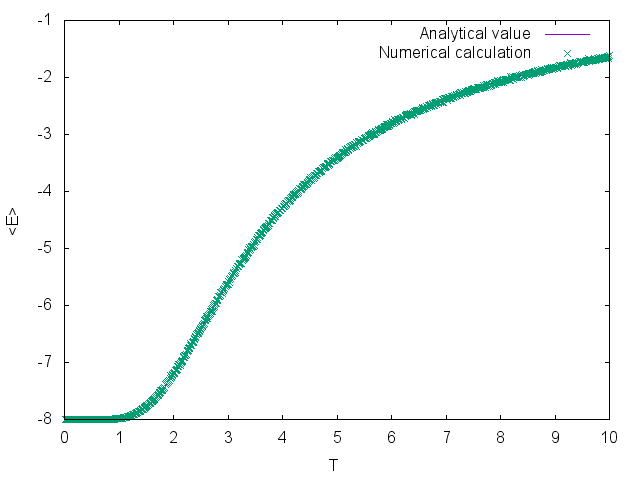
\includegraphics[width=\textwidth]{Energy.png}
	\caption{$<E>$ in a $2\times 2$-lattice for different temperatures\label{b_E}}
\end{figure}
\begin{figure}[h]
	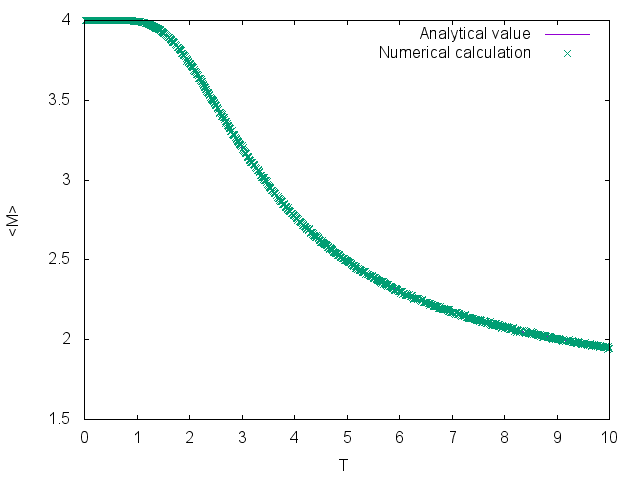
\includegraphics[width=\textwidth]{Magnetization.png}
	\caption{$<|M|>$ in a $2\times 2$-lattice for different temperatures\label{b_M}}
\end{figure}
\begin{figure}[h]
	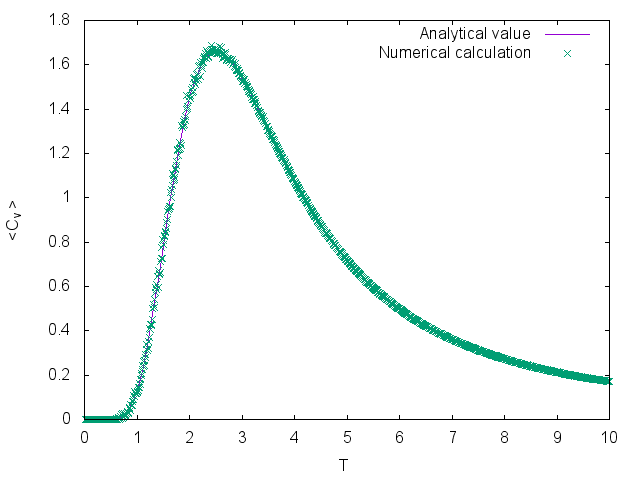
\includegraphics[width=\textwidth]{Heat_capacity.png}
	\caption{$<c_v>$ in a $2\times 2$-lattice for different temperatures\label{b_Cv}}
\end{figure}
\begin{figure}[h]
	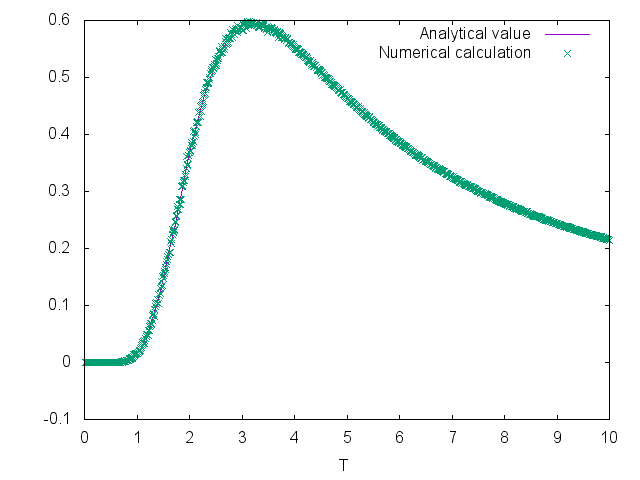
\includegraphics[width=\textwidth]{Susceptibility.png}
	\caption{$<\chi>$ in a $2\times 2$-lattice for different temperatures\label{b_chi}}
\end{figure}
In the next step, we took a closer look at the effect of thermalization. This term describes the process of the system slowly reaching the most likely state for a given temperature. When we start with a random setup, it is very unlikely that the system is already in this state at the beginning, but it will need some time (or, in our case, some Monte Carlo cycles) to reach it.

To get more insight in the process of thermalization, we observed the development of $<E>$ and $<|M|>$ of a $20\times20$-lattice for temperatures of $T=1.0$ and $T=2.4$, for both starting with a random setup and a lattice with all spins pointing in one direction. You can see that development in the figures \ref{c_1} -- \ref{c_4}, where these expectation values are plotted as function of the number of Monte Carlo cycles. We also plotted how many \glq moves\grq (flipping of spins) got accepted as a function of the number of cycles in fig. \ref{c_5} -- \ref{c_6} It is obvious that this value is proportional to the number of cycles and that, the higher the temperature is, the faster the number of accepted moves increases.

All these plots show that we need a bit more than $1000$ cycles in order to reach a stable state. This duration seems not to depend on the temperature, but obviously on the initial set-up: If this is close to a setup corresponding to the given temperature, it will not take long time to reach a stable state.

\label{results}
For later calculation, we set up a function called \emph{thermalization} for our program. This function performs the Metropolis algorithm without collecting data, instead it evaluates the energy after every 10 cycles. When the change between two measurements is less than $1\%$, the program starts collecting data. This takes in account the process described above and ensures that we reached a stable state before the actual calculations start.
\begin{figure}[h]
	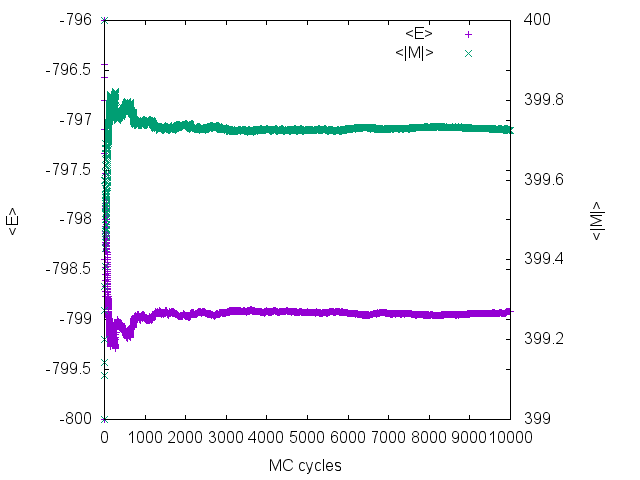
\includegraphics[width=\textwidth]{a1o.png}
	\caption{$<E>$ and $<|M|>$ in a $20\times 20$-lattice as a function of the number of Monte Carlo cycles, starting with ordered spins at $T=1.0$ \label{c_1}}
\end{figure}
\begin{figure}[h]
	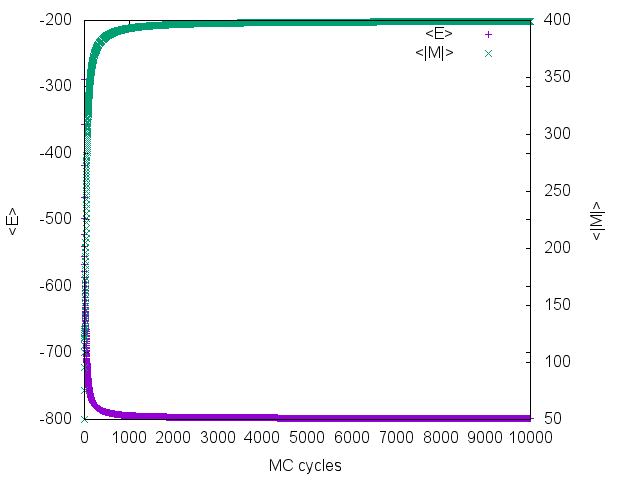
\includegraphics[width=\textwidth]{a1r.png}
	\caption{$<E>$ and $<|M|>$ in a $20\times 20$-lattice as a function of the number of Monte Carlo cycles, starting with random spins at $T=1.0$\label{c_2}}
\end{figure}
\begin{figure}[h]
	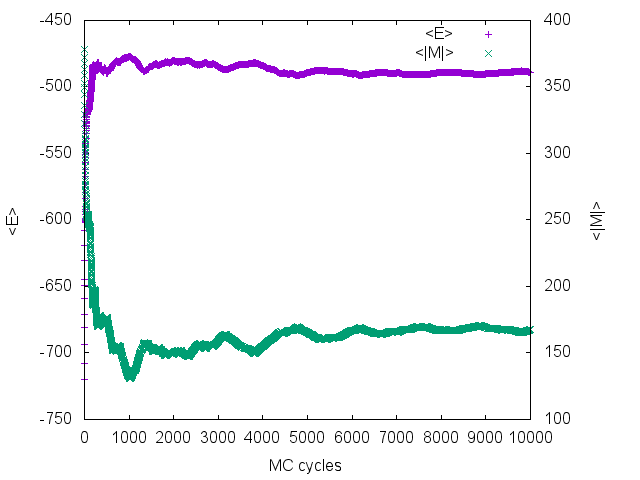
\includegraphics[width=\textwidth]{a24o.png}
	\caption{$<E>$ and $<|M|>$ in a $20\times 20$-lattice as a function of the number of Monte Carlo cycles, starting with ordered spins at $T=2.4$\label{c_3}}
\end{figure}
\begin{figure}[h]
	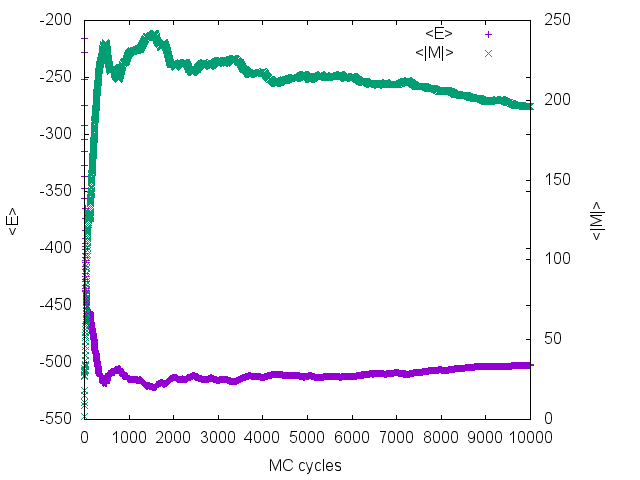
\includegraphics[width=\textwidth]{a24r.png}
	\caption{$<E>$ and $<|M|>$ in a $20\times 20$-lattice as a function of the number of Monte Carlo cycles, starting with random spins at $T=2.4$\label{c_4}}
\end{figure}

\begin{figure}[h]
	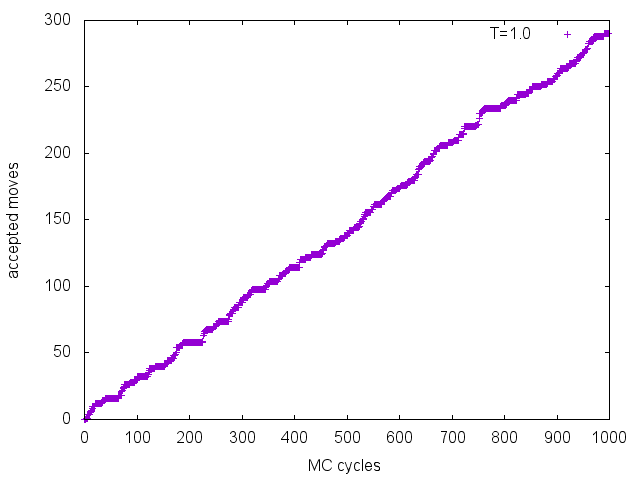
\includegraphics[width=\textwidth]{b1.png}
	\caption{The number of accepted spin flips as function of the number of cycles at $T=1.0$\label{c_5}}
\end{figure}
\begin{figure}[h]
	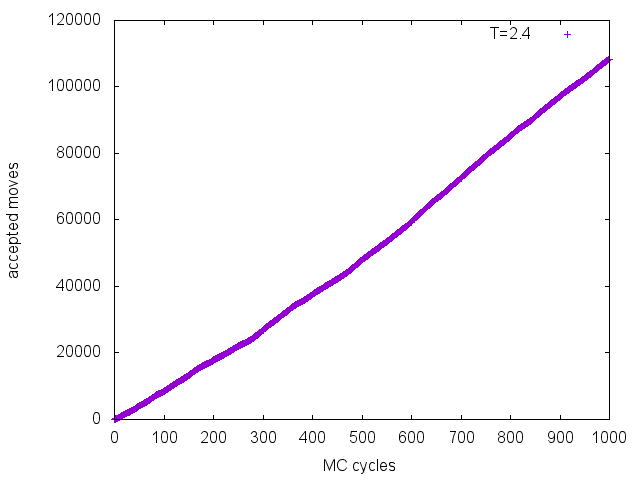
\includegraphics[width=\textwidth]{b24.png}
	\caption{The number of accepted spin flips as function of the number of cycles at $T=2.4$\label{c_6}}
\end{figure}

In the next step, we took a closer look at the probability of the single values of $E$ to appear. We observed a $2\times2$-lattice at a temperature of $T=1.0$ respectively $T=2.4$ again and did two histograms of how often an energy value occurred. Obviously, that distribution is expanded for a higher temperature. This correspondents with the fact that the variation of the energy for these temperatures is higher, which means that more values are accessed. Both histograms can be found in fig \ref{d1} -- \ref{d2}.

\begin{figure}[h]
	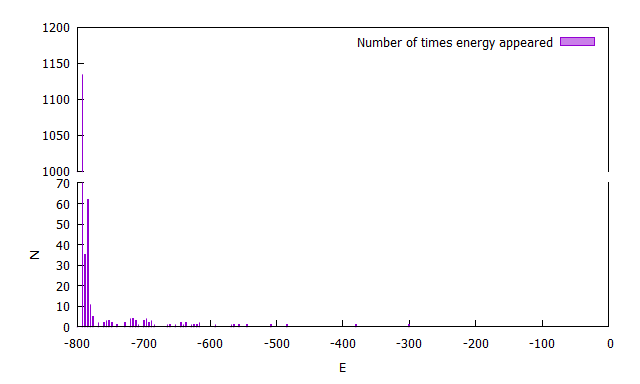
\includegraphics[width=\textwidth]{d1.png}
	\caption{Frequency of occurrence for different energies at $T=1.0$\label{d1}}
\end{figure}
\begin{figure}[h]
	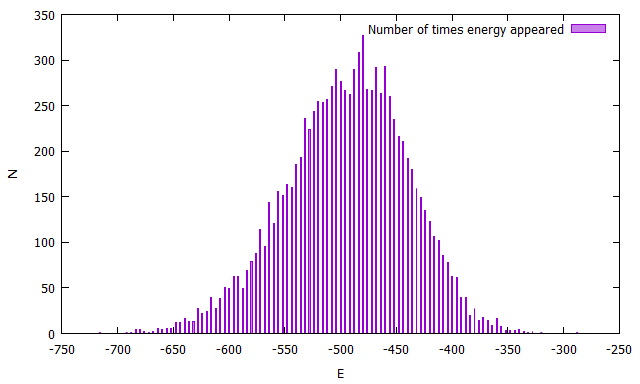
\includegraphics[width=\textwidth]{d24.png}
	\caption{Frequency of occurrence for different energies at $T=2.4$\label{d2}}
\end{figure}
\section{Comparison and discussion of results}

\section{source code}

\end{document}
